% Metódy inžinierskej práce

\documentclass[10pt,twoside,slovak,a4paper]{article}

\usepackage[slovak]{babel}
%\usepackage[T1]{fontenc}
\usepackage[IL2]{fontenc} % lepšia sadzba písmena Ľ než v T1
\usepackage[utf8]{inputenc}
\usepackage{graphicx}
\usepackage{url} % príkaz \url na formátovanie URL
\usepackage{hyperref} % odkazy v texte budú aktívne (pri niektorých triedach dokumentov spôsobuje posun textu)
\usepackage[final]{pdfpages}
\usepackage{cite}
%\usepackage{times}

\pagestyle{myheadings}

\title{Budúcnosť školských tried\thanks{Semestrálny projekt v predmete Metódy inžinierskej práce, ak. rok 2020/21, vedenie: Ing. Fedor Lehocki, PhD.}} % meno a priezvisko vyučujúceho na cvičeniach

\author{Marek Sunega\\[2pt]
	{\small Slovenská technická univerzita v Bratislave}\\
	{\small Fakulta informatiky a informačných technológií}\\
	{\small \texttt{xsunegam@stuba.sk}}
	}

\date{\small 30. september 2015} % upravte



\begin{document}

\maketitle

\begin{abstract}
    V článku sa uvádza ako by mohla vypadať virtuálna trieda vzhľadom na špecifika výučby počas 
	prebiehajúcej pandémie COVID 19. Zisťuje výhody a nevýhody a odprezentuváva ich. Zameriava 
	sa na rôzne typy virtuálnych tried a ich diferencie. Ukazuje hlavné rozdiely medzi tradičnou 
	a virtuálnou výučbou a porovnáva ich efektívnosť. Či by to niečo znamenalo pre klasické vyučovanie 
	a ako veľmi by sa dala virtuálna výučba automatizovať. Dala by sa virtuálna výučba ešte viac 
	využívať ako dnes a ci má nejakú budúcnosť. Uvádza výhody a vplyvy na učiteľov, žiakov, na ich 
	výsledky a efektivitu učenia.
\end{abstract}



\section{Úvod}
Prebiehajúca pandémia COVID-19 priniesla mnoho otázok aj do oblasti vzdelania. Obmedzilo sa vyučovanie, zaviedli 
opatrenia neskor sa školy úplne uzatvorili, prišla dištančná výučba.
Mnoho ľudí by mohlo mať sklon ospravedlňovať dištančné vzdelávanie jednoduchou otázkou: „Prečo nie?“.\cite{ency}
Existujú však dobré dôvody na to, aby ste diskutovali o tom, či je dištančné vzdelávanie oprávnené a aké sú 
jeho výhody vo vzťahu ku tradičnému vyučovaniu. Na druhej strane existujú aj také, 
ktoré predpokladajú, že dištančné vyučovanie sa podstatne nelíši od fyzckého vyučovania a ak je výučba dobrá a 
je možné učiť na diaľku, mali by sme ju viesť takou formou. Taktiež existujú ľudia, ktorí si myslia, že pri dištančnej výučbe 
človek stratí osobný rozmer, aj keď to nie je potrebné pre samotné vyučovanie, čo sa môže  javiť ako nevyhnutné pre 
efektívne vyučovanie. Málo kto si vie teda predstaviť, že by dištančná vyučba nahradila tú tradičnú. 

(odkazovanie na sekcie WIP)

\section{Nejaká časť} \label{nejaka}

NO učenie dialkovo alebo na diaľku je úplne možné.\cite{ency} Stávalo sa to už dávno a stále sa to deje. Svätý Pavol na diaľku učil kresťanských veriacich,
ktorí boli v Ríme, Korinte atď. pomocou ručne písaných listov. Autori, vzdialení priestorovo a aj časovo, učia svojich 
čitateľov prostredníctvom tlačených kníh a článkov.Vyučovať je možné na diaľku prostredníctvom 
filmov, televízie a videa. A dnes môžeme prostredníctvom internetu učiť kohokoľvek, kedykoľvek a hoci kde na svete.


\section{Nástup virtualneho vzdelávania}\label{covid}

Pandémia COVID-19 uzavrela školy na celom kontinente a poslala učiteľov, zamestnancov a študentov domov, aby študovali a pracovali na diaľku.

Prvá fáza (február - marec 2020) zahŕňala rýchly prechod na dištančnú výučbu a virtuálne vzdelávanie podporované nástrojmi na
videokonferencie (t. J. Zoom, WebEx, Adobe Connect). Druhá fáza (apríl - júl 2020),
ktorá zahŕňa pridanie základných prvkov online vzdelávania do webových stránok a systémov riadenia výučby.\cite{covid}
Ďalšia fáza (august - december 2020) bude pravdepodobne charakterizované obdobím kedy by školy už mali byť pripravené.
V záverečnej fáze, ktorá nás zavedie do roku 2021, sa objaví „nová norma“ vzdelávania. Aj keď sa školy nakoniec vrátia k
tradičnému vyučovaniu v triede, lekcie, ktoré sme sa všetci v tomto historickom čase naučili, nás vyzvú k tomu, aby sme pouvažovali 
aj nad možnosťami e-learningu.


\section{Virtuále učebne v praxi} \label{3}
Pre lepšie predstavenie skúseností z dvadsiatich rokov používania virtuálnych učební 
v terciárnom vzdelávaní sú funkcie, dostupné vo väčšine prostredí virtuálnych učební, rozdelené do 
dvoch skupín.\cite{VCf}  Do prvej skupiny (bežné funkcie) patria funkcie súvisiace iba s emuláciou tradičnej triedy. 
Druhá skupina (pokročilé funkcie) sa skladá z funkcií a postupov presahujúcich tradičné učebne.
Tabuľka obsahuje obe kategórie.

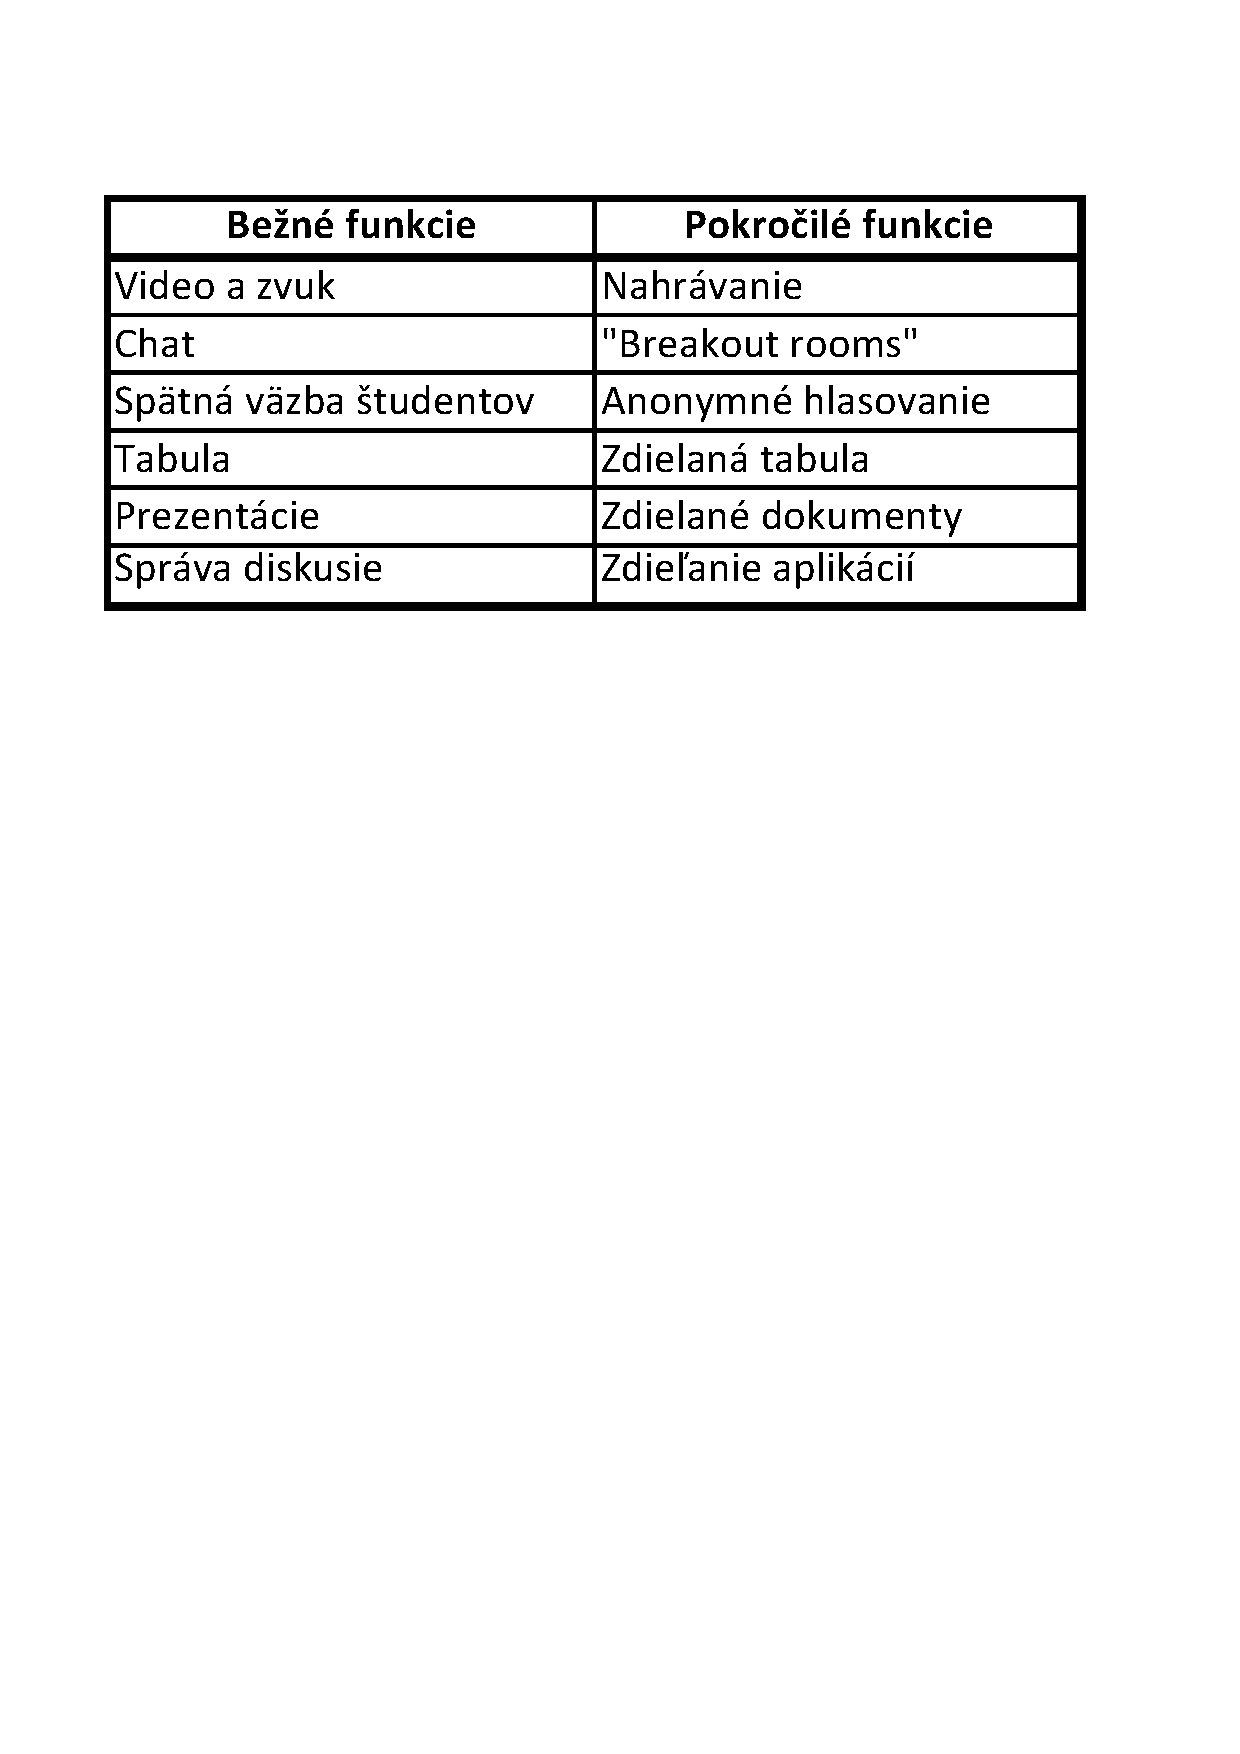
\includegraphics[width=\textwidth, trim = 0cm 15cm 0cm 2cm, clip]{tab1.pdf}\label{tab}



\subsection{Bežné funkcie pre napodobnenie klasickej triedy} \label{Bezne}

\begin{itemize}
\item V súčasnosti je \textbf{video a zvuk} k dispozícii pre profesora aj študentov.\cite{VCf} Osvedčeným postupom je pokúsiť sa,
aby sa všetci študenti prezentovali na videu, najmä v prípadoch, keď sa nestretli zoči-voči. Je pravda,
že pri dištančnom vzdelávaní je stretnutie študentov aspoň raz cenený pre budovanie komunity a v prípadoch,
keď to nie je možné, je nevyhnutné predstaviť sa pomocou videa a zvuku.

	\item Funkcia \textbf{četu} môže vždy pomôcť prekonať problémy so zvukom, a hoci nesúvisí s tradičnou praxou v triede, 
je uvedená v tomto zozname aj z historických, aj praktických dôvodov.\cite{VCf}Funkcia četu by okrem riešenia zvukových problémov 
mohla študentom umožniť lepšie objasniť otázku alebo umožniť profesorovi zbierať krátke odpovede, najmä ak chat podporuje 
priame správy medzi študentom a učiteľom, ako to robí väčšina súčasných virtualnych prostredí.

	\item \textbf{Správa diskusií} uľahčuje najnáročnejšiu úlohu,s ktoroú sa musí profesor vo virtuálnej učebne potrápiť.
Ovládanie publika s sledovanie „zdvihnutých rúk“  je niečo, čo si človek musí osvojiť v praxi.\cite{VCf}
\end{itemize}

\subsection{Pokročilé funkcie presahujúce tradičné učebne} \label{Pokr}
\begin{itemize}
	\item Funkcia \textbf{Breakout miestností} je veľmi užitočná pre zapojenie študentov.\cite{VCf}Sú užitočné na rozdelenie veľkej 
	skupiny do menších skupín, ktoré sa môžu rozprávať alebo spolupracovať. Existuje celý rad postupov 
	pri tímovej práci, ktoré by mohli využiť túto funkciu a jej správne použitie by skutočne mohlo vylepšiť 
	vzdelávací zážitok. Zatiaľ čo v typických učebniach je taká tímová práca vždy z hľadiska fyzikálnych obmedzení náročnejšia,
	vo virtuálnych učebniach sa dá niečo robiť s ľahkosťou. Osvedčeným postupom je zapojiť študentov pomerne často, počas virtuálnej hodiny (aspoň raz za každú hodinu),
	a nechať študentov, aby hlásili výsledky svoje diskusie späť v hlavnej miestnosti. \label{breakout}

	\item \textbf{Zdieľaná tabuľa} umožňuje študentom účasť na aktivitách súvisiacich s návrhovým schém,
	grafov a podobne. Profesor zvyčajne môže v hlavnej miestnosti požiadať viacerích dobrovoľníkov na raz o vypracovanie cvičenia
	alebo využiť na to už vyšie spomenute breakout miestnosti~\ref{breakout}, ktore umožnia rozdeliť študentov do viac miestnosti.

	\item \textbf{Zdieľanie dokumentov} a anotácií dovoluje profesorovi umožniť študentom spolupracovať na dokumente,
	napríklad kontrolovať kód a anotovať ako súčasť kolaboratívneho cvičenia.
	
\end{itemize}	
%\paragraph{Veľmi dôležitá poznámka.}
%Niekedy je potrebné nadpisom označiť odsek. Text pokračuje hneď za nadpisom.




\section{Záver} \label{zaver} % prípadne iný variant názvu
WIP


%\acknowledgement{Ak niekomu chcete poďakovať\ldots}


% týmto sa generuje zoznam literatúry z obsahu súboru literatura.bib podľa toho, na čo sa v článku odkazujete
\bibliography{lit}
\bibliographystyle{plain} % prípadne alpha, abbrv alebo hociktorý iný
\end{document}
